% Provenance (never printed): cycle 2 "Questionner l'espace et le temps"
% (the globe, the continents and the oceans, reading a world map); see
% sources/book1/PROVENANCE.md. Book 1, grade 3, chapter 2.
\chapter{ग्लोब: महाद्वीप और महासागर}\label{ch:g3:continents-and-oceans}

लीना की कक्षा में एक स्टैंड पर \omterm{def:g3:continents-and-oceans:globe}{ग्लोब} रखा है। लीना आँखें बंद करती है, एक
उँगली से उसे घुमाती है, और उँगली की नोक से उसे रोक देती है। वह आँखें खोलती
है: उसकी उँगली नीले रंग पर है, एक \omterm{def:g2:water-on-earth:ocean}{महासागर} के बीचोंबीच। वह फिर कोशिश करती
है: फिर नीला। तीसरी बार उसकी उँगली पीले-हरे रंग पर रुकती है, अफ़्रीका के
बीच में कहीं।

लीना खेलती रहती है, और गिनती है। उसकी उँगली ज़मीन से कहीं ज़्यादा बार
\omterm{def:g2:water-on-earth:ocean}{समुद्र} पर रुकती है। क्यों? और उसकी उँगली के नीचे घूमती ज़मीन और पानी की ये
सारी आकृतियाँ क्या हैं?

\begin{omfigure}
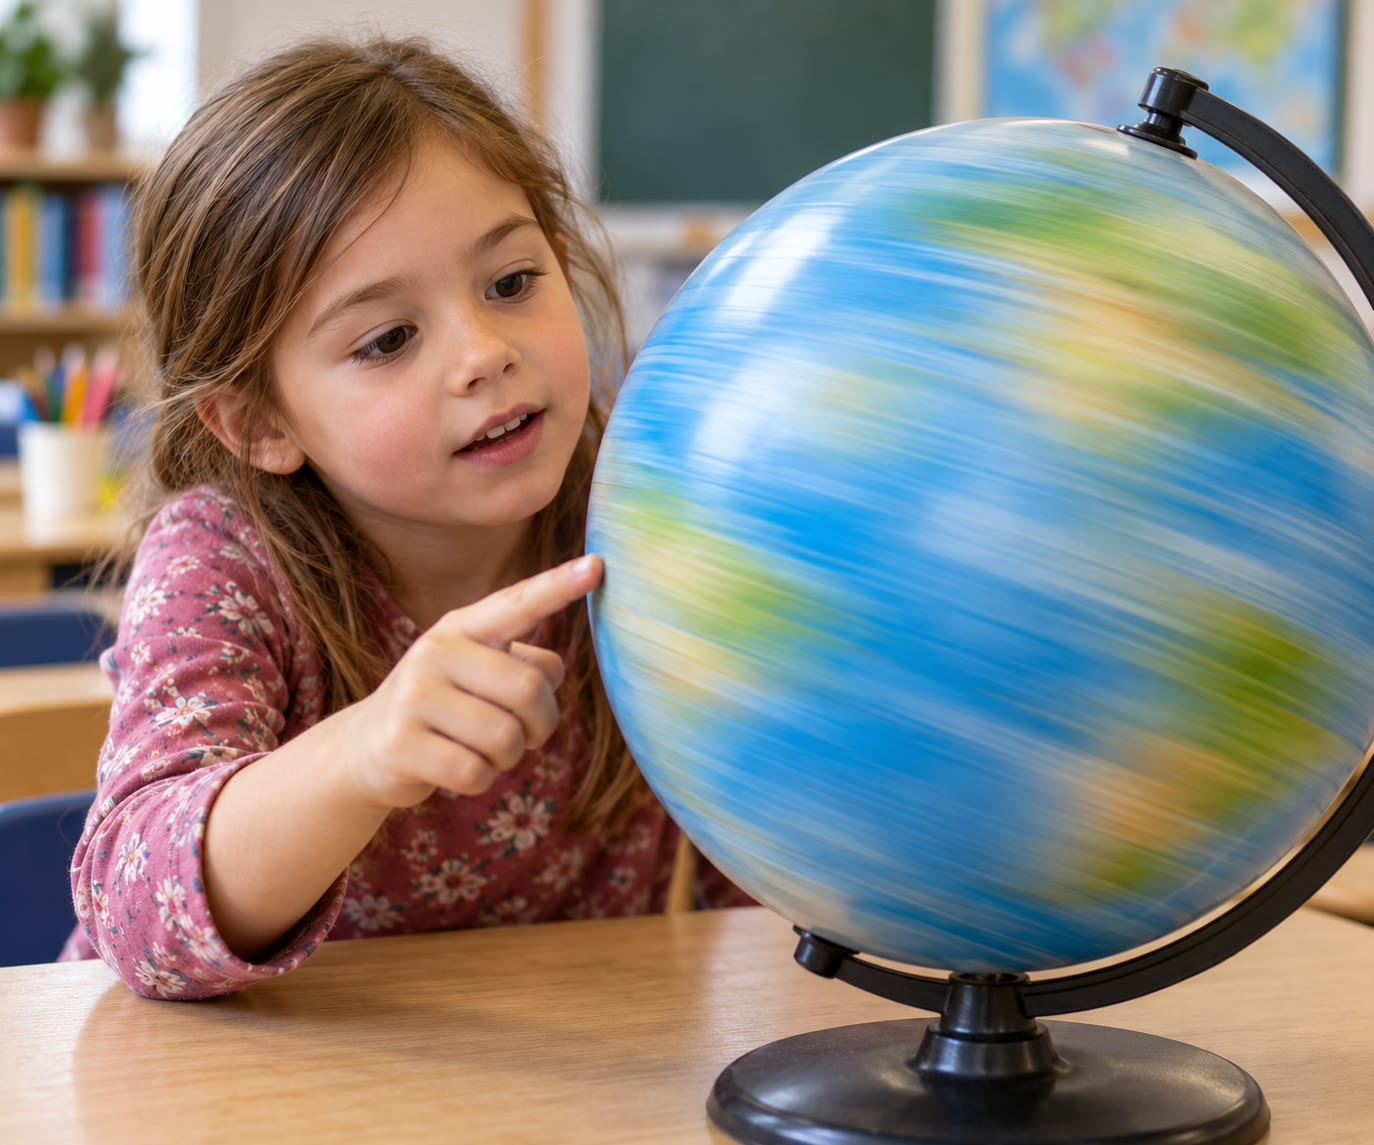
\includegraphics[width=0.6\linewidth]{images/book1/ai/g3-spinning-globe.jpg}

{\small अपने स्टैंड पर घूमता एक \omterm{def:g3:continents-and-oceans:globe}{ग्लोब}: उँगली के नीचे से ज़मीन और \omterm{def:g2:water-on-earth:ocean}{समुद्र}
गुज़रते जाते हैं।}
\end{omfigure}

\begin{recall}
पृथ्वी का ज़्यादातर भाग \omterm{def:g2:water-on-earth:salt-fresh}{खारे पानी} से ढका है: \cref{ch:g2:water-on-earth}
के जाल में 100 में से लगभग 71 वर्ग। \omterm{def:g2:water-on-earth:ocean}{महासागर} ज़मीन के बड़े टुकड़ों के बीच \omterm{def:g2:water-on-earth:salt-fresh}{खारे
पानी} का बहुत बड़ा फैलाव है; \omterm{def:g2:water-on-earth:ocean}{समुद्र} इससे छोटा फैलाव है, किसी \omterm{def:g2:water-on-earth:ocean}{महासागर} के
किनारे। \omterm{def:g2:drawing-to-map:map}{मानचित्र} किसी जगह का ऊपर से देखा हुआ, छोटा करके बनाया गया चित्र है
(\cref{ch:g2:drawing-to-map})। पृथ्वी दिन में एक बार अपने आप पर कैसे घूमती
है, जिससे दिन और रात होते हैं, यह भौतिकी की पुस्तकें बताती हैं।
\end{recall}

\section{ग्लोब, गोल पृथ्वी का एक छोटा मॉडल}

पृथ्वी गोल है, एक बहुत बड़ी गेंद की तरह। ज़मीन से हम उसका आकार नहीं देख
सकते, क्योंकि वह बहुत ही बड़ी है: हम कहीं भी खड़े हों, ज़मीन समतल दिखती है।
पर जो अंतरिक्ष-यात्री पृथ्वी से दूर गए, उन्होंने उसे पूरा देखा, काले आसमान
में एक गोल नीली गेंद (\cref{ch:g2:water-on-earth} की शुरुआत वाली तस्वीर)।

पूरी पृथ्वी को कक्षा में देखने के लिए हम उसे छोटा बना देते हैं।

\begin{definition}[ग्लोब]\label{def:g3:continents-and-oceans:globe}
\emph{ग्लोब}\index{ग्लोब} पृथ्वी का एक मॉडल है: एक गेंद, जिस पर ज़मीन और
\omterm{def:g2:water-on-earth:ocean}{महासागर} उन्हीं आकारों में बने हैं जैसे असली पृथ्वी पर, बस बहुत ही छोटे।
\end{definition}

\omterm{def:g3:continents-and-oceans:globe}{ग्लोब} पृथ्वी का सबसे अच्छा चित्र है, क्योंकि उसका आकार सही है: गोल। पर
असली पृथ्वी की तरह, हम एक बार में उसका सिर्फ़ आधा भाग देख पाते हैं। दूसरा
आधा देखने के लिए हम उसे घुमा देते हैं।

\begin{omfigure}
\begin{tikzpicture}
\begin{axis}[name=atl, hide axis, axis equal image, scale only axis,
    width=6.2cm, xmin=-1.05, xmax=1.05, ymin=-1.05, ymax=1.05, clip=false]
  \fill[omSea] (axis cs:0,0) circle[radius=1];
  \addplot[fill=omHypsLandA!85!black, draw=black!45, line width=0.2pt]
    table {figdata/out/grade-3-globe-atlantic-land.dat};
  \addplot[black!60, dashed, line width=0.5pt]
    table {figdata/out/grade-3-globe-atlantic-equator.dat};
  \addplot[only marks, mark=*, mark size=1.4pt, black]
    table[x=x, y=y] {figdata/out/grade-3-globe-atlantic-poles.dat};
  \node[font=\scriptsize, anchor=center, align=center, fill=white, fill opacity=0.7, text opacity=1, inner sep=1pt, rounded corners=1pt] at (axis cs:-0.683,0.636) {उत्तरी\\अमेरिका};
  \node[font=\scriptsize, anchor=center, align=center, fill=white, fill opacity=0.7, text opacity=1, inner sep=1pt, rounded corners=1pt] at (axis cs:-0.561,-0.408) {दक्षिणी\\अमेरिका};
  \node[font=\scriptsize, anchor=center, align=center, fill=white, fill opacity=0.7, text opacity=1, inner sep=1pt, rounded corners=1pt] at (axis cs:0.396,0.639) {यूरोप};
  \node[font=\scriptsize, anchor=center, align=center, fill=white, fill opacity=0.7, text opacity=1, inner sep=1pt, rounded corners=1pt] at (axis cs:0.704,-0.098) {अफ़्रीका};
  \node[font=\scriptsize, anchor=center, align=center, fill=white, fill opacity=0.7, text opacity=1, inner sep=1pt, rounded corners=1pt] at (axis cs:-0.209,0.128) {अटलांटिक\\महासागर};
  \draw[black!70, line width=0.8pt] (axis cs:0,0) circle[radius=1];
  \node[font=\scriptsize, anchor=south] at (axis cs:0,0.97) {उत्तरी ध्रुव};
\end{axis}
\begin{axis}[at={(atl.east)}, anchor=west, xshift=0.6cm, hide axis,
    axis equal image, scale only axis,
    width=6.2cm, xmin=-1.05, xmax=1.05, ymin=-1.05, ymax=1.05, clip=false]
  \fill[omSea] (axis cs:0,0) circle[radius=1];
  \addplot[fill=omHypsLandA!85!black, draw=black!45, line width=0.2pt]
    table {figdata/out/grade-3-globe-pacific-land.dat};
  \addplot[black!60, dashed, line width=0.5pt]
    table {figdata/out/grade-3-globe-pacific-equator.dat};
  \node[font=\scriptsize, anchor=center, align=center, fill=white, fill opacity=0.7, text opacity=1, inner sep=1pt, rounded corners=1pt] at (axis cs:-0.754,-0.391) {ऑस्ट्रेलिया};
  \node[font=\scriptsize, anchor=center, align=center, fill=white, fill opacity=0.7, text opacity=1, inner sep=1pt, rounded corners=1pt] at (axis cs:0.258,0.087) {प्रशांत\\महासागर};
  \draw[black!70, line width=0.8pt] (axis cs:0,0) circle[radius=1];
\end{axis}
\end{tikzpicture}

{\small दो ओर से देखा गया \omterm{def:g3:continents-and-oceans:globe}{ग्लोब}। बाएँ: अटलांटिक \omterm{def:g2:water-on-earth:ocean}{महासागर} वाली ओर, जिसमें दोनों
अमेरिका, यूरोप और अफ़्रीका हैं। दाएँ: दूसरी ओर, प्रशांत \omterm{def:g2:water-on-earth:ocean}{महासागर}, जिसके किनारे
पर ऑस्ट्रेलिया है। टूटी रेखा \omterm{def:g3:continents-and-oceans:equator}{भूमध्य रेखा} है। तटरेखाएँ: नैचुरल अर्थ
(सार्वजनिक डोमेन)।}
\label{fig:g3:continents-and-oceans:globes}
% ledger: data:ne-land
\end{omfigure}

\begin{remark}[दो बहुत अलग आधे भाग]\label{rem:g3:continents-and-oceans:halves}
दोनों चित्रों को देखो। बाएँ चित्र में ज़मीन चित्र के 10 में से लगभग 4 भाग
घेरती है। दाएँ चित्र में 10 में से सिर्फ़ लगभग 1 भाग: पृथ्वी की प्रशांत वाली
ओर लगभग पूरी पानी है। अगर लीना की उँगली \omterm{def:g3:continents-and-oceans:globe}{ग्लोब} की उस ओर रुके, तो वह लगभग
हमेशा \omterm{def:g2:water-on-earth:ocean}{समुद्र} पर ही पड़ेगी।
\end{remark}

\section{भूमध्य रेखा, ध्रुव और दो गोलार्ध}

\omterm{def:g3:continents-and-oceans:globe}{ग्लोब} एक छड़ पर घूमता है जो ऊपर से नीचे तक उसके आर-पार जाती है। असली पृथ्वी
में कोई छड़ नहीं है, पर वह भी अपने बीच से गुज़रने वाली एक रेखा के चारों ओर
घूमती है। जिन दो जगहों पर वह रेखा पृथ्वी से बाहर निकलती है, उनके नाम हैं।

\begin{definition}[ध्रुव]\label{def:g3:continents-and-oceans:poles}
\emph{उत्तरी ध्रुव}\index{उत्तरी ध्रुव} और \emph{दक्षिणी
ध्रुव}\index{दक्षिणी ध्रुव} पृथ्वी के बिलकुल ऊपर और बिलकुल नीचे के वे दो
बिंदु हैं जहाँ से वह रेखा बाहर निकलती है जिसके चारों ओर पृथ्वी घूमती है।
इनमें से हर एक \emph{ध्रुव}\index{ध्रुव} है। \omterm{def:g3:continents-and-oceans:globe}{ग्लोब} पर उत्तरी ध्रुव सबसे ऊपर
होता है।
\end{definition}

\begin{definition}[भूमध्य रेखा और गोलार्ध]\label{def:g3:continents-and-oceans:equator}
\emph{भूमध्य रेखा}\index{भूमध्य रेखा} पृथ्वी के चारों ओर पूरी खींची गई एक
काल्पनिक रेखा है, जो \omterm{def:g3:continents-and-oceans:poles}{उत्तरी ध्रुव} और \omterm{def:g3:continents-and-oceans:poles}{दक्षिणी ध्रुव} के ठीक बीचोंबीच है। वह
पृथ्वी को दो आधे भागों में काटती है, जिनमें से हर एक
\emph{गोलार्ध}\index{गोलार्ध} कहलाता है: \omterm{def:g3:continents-and-oceans:poles}{उत्तरी ध्रुव} की ओर
\emph{उत्तरी गोलार्ध}\index{उत्तरी गोलार्ध}, और \omterm{def:g3:continents-and-oceans:poles}{दक्षिणी ध्रुव} की ओर
\emph{दक्षिणी गोलार्ध}\index{दक्षिणी गोलार्ध}।
\end{definition}

\omterm{def:g3:continents-and-oceans:equator}{भूमध्य रेखा} ज़मीन पर रंगी हुई नहीं है: कोई उसे \omterm{def:g2:water-on-earth:ocean}{समुद्र} \omterm{def:g1:landscapes-around-us:water}{तट} पर या जंगल में नहीं
देख सकता। रास्ता ढूँढने में मदद के लिए उसे \omterm{def:g3:continents-and-oceans:globe}{ग्लोबों} और \omterm{def:g2:drawing-to-map:map}{मानचित्रों} पर बनाया
जाता है।

\begin{omfigure}
\begin{tikzpicture}[font=\small]
  % globe outline
  \fill[omSea!70] (0,0) circle (2.2);
  % northern hemisphere tinted
  \begin{scope}
    \clip (0,0) circle (2.2);
    \fill[yellow!25, opacity=0.8] (-2.3,0) -- (-2.3,2.3) -- (2.3,2.3) -- (2.3,0)
      arc[start angle=0, end angle=-180, x radius=2.3, y radius=0.45] -- cycle;
  \end{scope}
  \draw[black!70, line width=0.8pt] (0,0) circle (2.2);
  % equator: front half solid, back half dashed
  \draw[red!70!black, line width=1.2pt] (-2.2,0) arc[start angle=180, end angle=360, x radius=2.2, y radius=0.4];
  \draw[red!70!black, line width=0.8pt, dashed] (2.2,0) arc[start angle=0, end angle=180, x radius=2.2, y radius=0.4];
  % axis and poles
  \draw[black!60, line width=0.6pt] (0,2.2) -- (0,2.75);
  \draw[black!60, line width=0.6pt] (0,-2.2) -- (0,-2.75);
  \draw[black!60, line width=0.6pt, dotted] (0,2.2) -- (0,-2.2);
  \fill (0,2.2) circle (2.2pt);
  \fill (0,-2.2) circle (2.2pt);
  \node[anchor=west] at (0.15,2.6) {उत्तरी ध्रुव};
  \node[anchor=west] at (0.15,-2.6) {दक्षिणी ध्रुव};
  % labels
  \node[anchor=west] at (2.6,0) {भूमध्य रेखा};
  \draw[black!60] (2.55,0) -- (2.05,-0.15);
  \node[anchor=west, align=left] at (2.6,1.4) {उत्तरी\\गोलार्ध};
  \draw[black!60] (2.55,1.4) -- (1.5,1.2);
  \node[anchor=west, align=left] at (2.6,-1.4) {दक्षिणी\\गोलार्ध};
  \draw[black!60] (2.55,-1.4) -- (1.5,-1.2);
\end{tikzpicture}

{\small \omterm{def:g3:continents-and-oceans:equator}{भूमध्य रेखा} पृथ्वी को दो \omterm{def:g3:continents-and-oceans:equator}{गोलार्धों} में काटती है। \omterm{def:g3:continents-and-oceans:equator}{उत्तरी गोलार्ध} (रंगा
हुआ) \omterm{def:g3:continents-and-oceans:poles}{उत्तरी ध्रुव} की ओर है, \omterm{def:g3:continents-and-oceans:equator}{दक्षिणी गोलार्ध} \omterm{def:g3:continents-and-oceans:poles}{दक्षिणी ध्रुव} की ओर।}
\label{fig:g3:continents-and-oceans:hemispheres}
\end{omfigure}

\begin{example}[भूमध्य रेखा के पास गरम, ध्रुवों के पास ठंडा]\label{ex:g3:continents-and-oceans:hot-cold}
\omterm{def:g3:continents-and-oceans:equator}{भूमध्य रेखा} के पास के इलाक़े साल भर गरम रहते हैं: वहीं बड़े वर्षावन उगते
हैं। \omterm{def:g3:continents-and-oceans:poles}{ध्रुवों} के पास के इलाक़े साल भर ठंडे रहते हैं, और उनका बड़ा भाग बर्फ़ से
ढका है। ऐसा क्यों है, यह तुम आगे की किसी कक्षा में सीखोगे; अभी के लिए याद
रखो: \omterm{def:g3:continents-and-oceans:poles}{ध्रुव} के जितना पास, उतनी ज़्यादा ठंड।
\end{example}

\section{सात महाद्वीप और पाँच महासागर}

\omterm{def:g3:continents-and-oceans:globe}{ग्लोब} पर ज़मीन हर जगह छोटे-छोटे टुकड़ों में बिखरी नहीं है। उसका ज़्यादातर भाग
कुछ बहुत बड़े भूभागों में इकट्ठा है।

\begin{definition}[महाद्वीप]\label{def:g3:continents-and-oceans:continent}
\emph{महाद्वीप}\index{महाद्वीप} पृथ्वी पर ज़मीन के बहुत बड़े भूभागों में से
एक है, अपने पास के द्वीपों के साथ।
\end{definition}

लोग ज़्यादातर सात \omterm{def:g3:continents-and-oceans:continent}{महाद्वीप} गिनते हैं। सबसे बड़े से सबसे छोटे तक वे हैं:
एशिया, अफ़्रीका, उत्तरी अमेरिका, दक्षिणी अमेरिका, अंटार्कटिका, यूरोप और
ऑस्ट्रेलिया।
% ledger: natgeo:seven-continents

\begin{center}\small
\begin{tabular}{rlll}
\hline
आकार & \omterm{def:g3:continents-and-oceans:continent}{महाद्वीप} & \omterm{def:g3:continents-and-oceans:equator}{गोलार्ध} & इसके बारे में एक बात \\
\hline
1 & एशिया & ज़्यादातर उत्तरी & सबसे बड़ा \\
2 & अफ़्रीका & दोनों & \omterm{def:g3:continents-and-oceans:equator}{भूमध्य रेखा} इसके बीच से गुज़रती है \\
3 & उत्तरी अमेरिका & उत्तरी & उत्तर में बहुत दूर तक जाता है \\
4 & दक्षिणी अमेरिका & ज़्यादातर दक्षिणी & \omterm{def:g3:continents-and-oceans:equator}{भूमध्य रेखा} इसके उत्तरी भाग से गुज़रती है \\
5 & अंटार्कटिका & दक्षिणी & \omterm{def:g3:continents-and-oceans:poles}{दक्षिणी ध्रुव} के चारों ओर, बर्फ़ के नीचे \\
6 & यूरोप & उत्तरी & अपनी पूर्वी ओर एशिया से जुड़ा \\
7 & ऑस्ट्रेलिया & दक्षिणी & सबसे छोटा \\
\hline
\end{tabular}
\end{center}

\begin{remark}[एक महाद्वीप कहाँ ख़त्म होता है?]\label{rem:g3:continents-and-oceans:where}
कुछ \omterm{def:g3:continents-and-oceans:continent}{महाद्वीप} हर ओर से \omterm{def:g2:water-on-earth:ocean}{समुद्र} से घिरे हैं, जैसे ऑस्ट्रेलिया या अंटार्कटिका।
दूसरे आपस में मिले हुए हैं: यूरोप और एशिया ज़मीन का एक ही भूभाग हैं, और
उनके बीच की रेखा कहाँ खींची जाए, यह लोगों ने चुना। इसीलिए कुछ लोग छह
\omterm{def:g3:continents-and-oceans:continent}{महाद्वीप} गिनते हैं, या इससे भी कम।
\end{remark}

\omterm{def:g3:continents-and-oceans:continent}{महाद्वीपों} के बीच \omterm{def:g2:water-on-earth:ocean}{महासागर} हैं। वे पाँच हैं। सबसे बड़ा \emph{प्रशांत
\omterm{def:g2:water-on-earth:ocean}{महासागर}} है; फिर आते हैं \emph{अटलांटिक \omterm{def:g2:water-on-earth:ocean}{महासागर}}, \emph{हिंद \omterm{def:g2:water-on-earth:ocean}{महासागर}},
अंटार्कटिका के चारों ओर \emph{दक्षिणी \omterm{def:g2:water-on-earth:ocean}{महासागर}}, और सबसे छोटा, \omterm{def:g3:continents-and-oceans:poles}{उत्तरी ध्रुव} के
चारों ओर \emph{आर्कटिक \omterm{def:g2:water-on-earth:ocean}{महासागर}}। बहुत समय तक लोग सिर्फ़ चार गिनते थे; आज
ज़्यादातर देश दक्षिणी \omterm{def:g2:water-on-earth:ocean}{महासागर} को पाँचवाँ गिनते हैं।
% ledger: nos:five-oceans, nos:pacific-largest, oer:arctic-smallest

\begin{example}[प्रशांत महासागर कितना बड़ा है?]\label{ex:g3:continents-and-oceans:pacific}
प्रशांत \omterm{def:g2:water-on-earth:ocean}{महासागर} इतना बड़ा है कि सारे \omterm{def:g3:continents-and-oceans:continent}{महाद्वीप} मिलाकर भी उसके अंदर समा सकते
हैं। पृथ्वी के सारे \omterm{def:g2:water-on-earth:ocean}{महासागरों} के पानी का आधे से ज़्यादा भाग उसी में है। इसीलिए
इस अध्याय के पहले अनुभाग में दाईं ओर वाला \omterm{def:g3:continents-and-oceans:globe}{ग्लोब} लगभग पूरा नीला दिखता है।
% ledger: nos:pacific-largest
\end{example}

\begin{method}[दो महाद्वीपों के बीच के महासागर का नाम बताना]\label{met:g3:continents-and-oceans:between}
दो \omterm{def:g3:continents-and-oceans:continent}{महाद्वीपों} के बीच कौन-सा \omterm{def:g2:water-on-earth:ocean}{महासागर} है, यह जानने के लिए \omterm{def:g3:continents-and-oceans:globe}{ग्लोब} पर दोनों पर
एक-एक उँगली रखो, और \omterm{def:g3:continents-and-oceans:globe}{ग्लोब} को ऐसे घुमाओ कि दोनों दिखें। एक उँगली से दूसरी तक
जाने में तुम्हारी नज़र जो \omterm{def:g2:water-on-earth:ocean}{महासागर} पार करती है, वही उनके बीच का \omterm{def:g2:water-on-earth:ocean}{महासागर} है।
\omterm{def:g3:continents-and-oceans:globe}{ग्लोब} पर अक्सर घूमकर जाने के दो रास्ते होते हैं: छोटा वाला लो।
\end{method}

\begin{example}[अफ़्रीका और ऑस्ट्रेलिया]\label{ex:g3:continents-and-oceans:africa-australia}
अफ़्रीका से पूर्व की ओर ऑस्ट्रेलिया जाते हुए हम हिंद \omterm{def:g2:water-on-earth:ocean}{महासागर} पार करते हैं।
यूरोप से पश्चिम की ओर उत्तरी अमेरिका जाते हुए हम अटलांटिक \omterm{def:g2:water-on-earth:ocean}{महासागर} पार करते
हैं। एशिया से पूर्व की ओर उत्तरी अमेरिका जाते हुए हम प्रशांत \omterm{def:g2:water-on-earth:ocean}{महासागर} पार करते हैं।
\end{example}

\section{विश्व मानचित्र एक चपटा किया गया ग्लोब है}

\omterm{def:g3:continents-and-oceans:globe}{ग्लोब} गोल है, इसलिए उसे साथ ले जाना आसान नहीं, और हम उसे कभी एक साथ पूरा
नहीं देख सकते। काग़ज़ के पन्ने पर बना \omterm{def:g2:drawing-to-map:map}{मानचित्र} पूरी पृथ्वी को एक नज़र में
दिखा देता है।

\begin{definition}[विश्व मानचित्र]\label{def:g3:continents-and-oceans:world-map}
\emph{विश्व मानचित्र}\index{विश्व मानचित्र} पूरी पृथ्वी का \omterm{def:g2:drawing-to-map:map}{मानचित्र} है जो
काग़ज़ के पन्ने या किसी स्क्रीन पर चपटा बनाया जाता है, जिसमें सारे \omterm{def:g3:continents-and-oceans:continent}{महाद्वीप}
और सारे \omterm{def:g2:water-on-earth:ocean}{महासागर} एक ही चित्र में होते हैं।
\end{definition}

\begin{omfigure}
\begin{tikzpicture}
\begin{axis}[ommap, width=\linewidth, xtick=\empty, ytick={0},
    yticklabels={भूमध्य रेखा}, grid=none, clip=true]
  \addplot[fill=omHypsLandA!85!black, draw=black!45, line width=0.2pt]
    table {figdata/out/shared-geo-land.dat};
  \draw[black!60, dashed, line width=0.5pt] (axis cs:-180,0) -- (axis cs:180,0);
  \begin{scope}[every node/.style={font=\scriptsize, align=center}]
    \node at (axis cs:-102,47) {उत्तरी\\अमेरिका};
    \node at (axis cs:-60,-12) {दक्षिणी\\अमेरिका};
    \node at (axis cs:17,52) {यूरोप};
    \node at (axis cs:20,6) {अफ़्रीका};
    \node at (axis cs:92,48) {एशिया};
    \node at (axis cs:134,-24) {ऑस्ट्रेलिया};
    \node at (axis cs:40,-80) {अंटार्कटिका};
  \end{scope}
  \begin{scope}[every node/.style={font=\scriptsize\itshape, align=center, text=omSea!35!black}]
    \node at (axis cs:-145,8) {प्रशांत\\महासागर};
    \node at (axis cs:165,12) {प्रशांत\\महासागर};
    \node at (axis cs:-38,22) {अटलांटिक\\महासागर};
    \node at (axis cs:-15,-25) {अटलांटिक\\महासागर};
    \node at (axis cs:78,-22) {हिंद\\महासागर};
    \node at (axis cs:-115,-57) {दक्षिणी महासागर};
    \node at (axis cs:-150,79) {आर्कटिक महासागर};
  \end{scope}
\end{axis}
\end{tikzpicture}

{\small एक \omterm{def:g3:continents-and-oceans:world-map}{विश्व मानचित्र}। \omterm{def:g3:continents-and-oceans:globe}{ग्लोब} को प्रशांत \omterm{def:g2:water-on-earth:ocean}{महासागर} के बीच से गुज़रने वाली एक
रेखा पर काटकर फैलाकर चपटा किया गया है: प्रशांत \omterm{def:g2:water-on-earth:ocean}{महासागर} दो बार दिखता है, बाएँ
और दाएँ किनारे पर। अंटार्कटिका, \omterm{def:g3:continents-and-oceans:poles}{दक्षिणी ध्रुव} के चारों ओर का एक गोल \omterm{def:g3:continents-and-oceans:continent}{महाद्वीप},
नीचे के किनारे पर एक लंबी पट्टी की तरह खिंच गया है।
तटरेखाएँ: नैचुरल अर्थ (सार्वजनिक डोमेन)।}
\label{fig:g3:continents-and-oceans:world-map}
% ledger: data:ne-land
\end{omfigure}

पर एक मुश्किल है। किसी संतरे के छिलके को मेज़ पर चपटा करके देखो: वह फटे या
खिंचे बिना सपाट नहीं हो सकता। \omterm{def:g3:continents-and-oceans:globe}{ग्लोब} की सतह को चपटा बनाने पर उसके साथ भी यही
होता है। हर \omterm{def:g3:continents-and-oceans:world-map}{विश्व मानचित्र} \omterm{def:g3:continents-and-oceans:globe}{ग्लोब} को कहीं न कहीं फाड़ता है, या कुछ जगहों को
खींचता और कुछ को दबाता है।

\begin{omfigure}
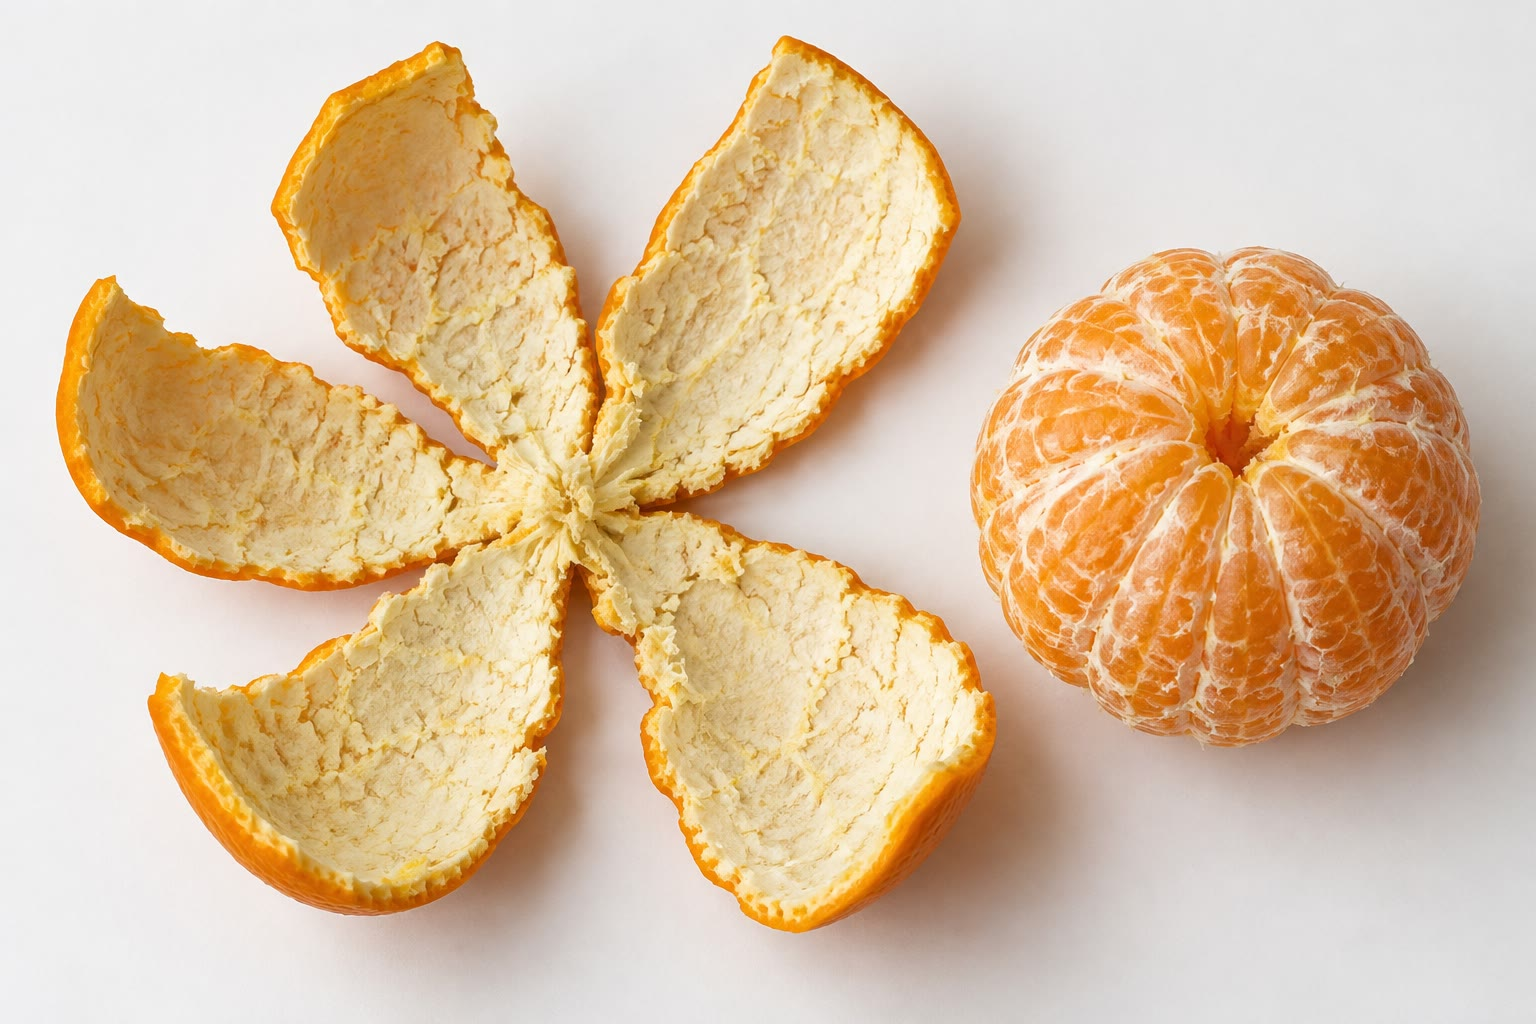
\includegraphics[width=0.4\linewidth]{images/book1/ai/g3-orange-peel.jpg}

{\small संतरे का छिलका फटे बिना सपाट नहीं हो सकता।}
\end{omfigure}

\begin{remark}[मानचित्र और ग्लोब में अंतर]\label{rem:g3:continents-and-oceans:disagree}
इस \omterm{def:g3:continents-and-oceans:world-map}{विश्व मानचित्र} पर अंटार्कटिका सबसे बड़े \omterm{def:g3:continents-and-oceans:continent}{महाद्वीपों} में से एक लगता है, नीचे
के पूरे किनारे पर खिंचा हुआ। \omterm{def:g3:continents-and-oceans:globe}{ग्लोब} पर वह ज़मीन का एक गोल भूभाग है, दक्षिणी
अमेरिका से छोटा। \omterm{def:g3:continents-and-oceans:poles}{ध्रुवों} के पास चपटा \omterm{def:g2:drawing-to-map:map}{मानचित्र} ज़मीन को बहुत खींच देता है।
\omterm{def:g3:continents-and-oceans:equator}{भूमध्य रेखा} के पास वह उसे बहुत कम खींचता है। जब तुम \omterm{def:g3:continents-and-oceans:equator}{भूमध्य रेखा} से दूर की दो
जगहों के आकार की तुलना करना चाहो, तो \omterm{def:g3:continents-and-oceans:globe}{ग्लोब} सच बताता है।
\end{remark}

\begin{method}[विश्व मानचित्र पढ़ना]\label{met:g3:continents-and-oceans:reading}
इस जैसे \omterm{def:g3:continents-and-oceans:world-map}{विश्व मानचित्र} पर:
\begin{enumerate}
  \item उत्तर सबसे ऊपर है, दक्षिण सबसे नीचे; \omterm{def:g3:continents-and-oceans:poles}{उत्तरी ध्रुव} पूरा ऊपरी किनारा
        है और \omterm{def:g3:continents-and-oceans:poles}{दक्षिणी ध्रुव} पूरा निचला किनारा;
  \item \omterm{def:g3:continents-and-oceans:equator}{भूमध्य रेखा} बीच में से जाने वाली रेखा है: उसके ऊपर का सब कुछ \omterm{def:g3:continents-and-oceans:equator}{उत्तरी
        गोलार्ध} में है, उसके नीचे का सब कुछ \omterm{def:g3:continents-and-oceans:equator}{दक्षिणी गोलार्ध} में;
  \item बायाँ और दायाँ किनारा \omterm{def:g3:continents-and-oceans:globe}{ग्लोब} पर एक ही रेखा हैं: जो जहाज़ दाएँ किनारे
        से बाहर निकलता है, वह बाएँ किनारे पर लौट आता है।
\end{enumerate}
\end{method}

\section{अभ्यास}

\begin{exercise}[$\star$]\label{exo:g3:continents-and-oceans:1}
सातों \omterm{def:g3:continents-and-oceans:continent}{महाद्वीपों} के नाम बताओ। सबसे बड़ा कौन-सा है? सबसे छोटा कौन-सा?
\end{exercise}

\begin{exercise}[$\star$]\label{exo:g3:continents-and-oceans:2}
पाँचों \omterm{def:g2:water-on-earth:ocean}{महासागरों} के नाम बताओ। सबसे बड़ा कौन-सा है? सबसे छोटा कौन-सा?
\end{exercise}

\begin{exercise}[$\star$]\label{exo:g3:continents-and-oceans:3}
``\omterm{def:g3:continents-and-oceans:poles}{उत्तरी ध्रुव}'', ``\omterm{def:g3:continents-and-oceans:poles}{दक्षिणी ध्रुव}'' या ``\omterm{def:g3:continents-and-oceans:equator}{भूमध्य रेखा}'' से भरकर उतारो:
\dots{} \omterm{def:g3:continents-and-oceans:globe}{ग्लोब} के सबसे ऊपर है; \dots{} सबसे नीचे है; \dots{} बीच में
पूरा चक्कर लगाती है।
\end{exercise}

\begin{exercise}[$\star$]\label{exo:g3:continents-and-oceans:4}
\omterm{def:g3:continents-and-oceans:equator}{उत्तरी गोलार्ध} या \omterm{def:g3:continents-and-oceans:equator}{दक्षिणी गोलार्ध}? यूरोप; ऑस्ट्रेलिया; अंटार्कटिका; उत्तरी
अमेरिका।
\end{exercise}

\begin{exercise}[$\star$]\label{exo:g3:continents-and-oceans:5}
\omterm{def:g3:continents-and-oceans:poles}{उत्तरी ध्रुव} के चारों ओर कौन-सा \omterm{def:g2:water-on-earth:ocean}{महासागर} है? अंटार्कटिका के चारों ओर कौन-सा
\omterm{def:g2:water-on-earth:ocean}{महासागर} है?
\end{exercise}

\begin{exercise}[$\star\star$]\label{exo:g3:continents-and-oceans:6}
अफ़्रीका से दक्षिणी अमेरिका जाने के लिए तुम कौन-सा \omterm{def:g2:water-on-earth:ocean}{महासागर} पार करते हो?
ऑस्ट्रेलिया से दक्षिणी अमेरिका, पूर्व की ओर जाते हुए? अफ़्रीका से ऑस्ट्रेलिया?
\end{exercise}

\begin{exercise}[$\star\star$]\label{exo:g3:continents-and-oceans:7}
सैम ऐसे देश में रहता है जहाँ साल भर गरमी रहती है। बो एक अनुसंधान केंद्र पर
रहती है जहाँ साल भर कड़ाके की ठंड रहती है। इनमें से एक \omterm{def:g3:continents-and-oceans:equator}{भूमध्य रेखा} के पास
रहता है, दूसरा किसी \omterm{def:g3:continents-and-oceans:poles}{ध्रुव} के पास। कौन कहाँ रहता है?
\end{exercise}

\begin{exercise}[$\star\star$]\label{exo:g3:continents-and-oceans:8}
लीना \omterm{def:g3:continents-and-oceans:globe}{ग्लोब} को 10 बार घुमाती है। उसकी उँगली 7 बार \omterm{def:g2:water-on-earth:ocean}{समुद्र} पर पड़ती है। कितनी
बार वह ज़मीन पर पड़ती है? क्या तुमने यही सोचा था? क्यों?
\end{exercise}

\begin{exercise}[$\star\star$]\label{exo:g3:continents-and-oceans:9}
पृष्ठ~\pageref{fig:g3:continents-and-oceans:world-map} के \omterm{def:g3:continents-and-oceans:world-map}{विश्व मानचित्र} पर
प्रशांत \omterm{def:g2:water-on-earth:ocean}{महासागर} दो बार दिखता है। क्यों? क्या असली पृथ्वी पर दो प्रशांत
\omterm{def:g2:water-on-earth:ocean}{महासागर} हैं?
\end{exercise}

\begin{exercise}[$\star\star\star$]\label{exo:g3:continents-and-oceans:10}
टॉम कहता है: ``\omterm{def:g3:continents-and-oceans:world-map}{विश्व मानचित्र} पर अंटार्कटिका एशिया से लंबा है, इसलिए
अंटार्कटिका सबसे बड़ा \omterm{def:g3:continents-and-oceans:continent}{महाद्वीप} है।'' क्या टॉम सही है? \omterm{def:g3:continents-and-oceans:continent}{महाद्वीपों} की सबसे बड़े
से सबसे छोटे तक की सूची का इस्तेमाल करो, और बताओ कि \omterm{def:g3:continents-and-oceans:world-map}{विश्व मानचित्र} उसे धोखा
क्यों देता है।
\end{exercise}
